\chapter{Legal and Ethical aspects of Privacy}
\label{chap:privacy}

As privacy is a very general and hard to grasp term, we need to fix a definition of privacy that is suitable for our needs.
As background information we include an overview about historical treatments of privacy as well as legal regulation of privacy in the European Union.
Based on this we propose a definition of privacy as {\em control over personal data}, and introduce a taxonomy of privacy attributes that give specify the term {\em personal data} in the context of mobile sensor data collection.

\section{Histrocial Approaches to Privacy}

\subsection{Aristotle}

Public Sphere vs. Private Sphere of politics. This distinction is concerned with the politic (public) life of politicians in early democracies opposed by their domestic (private) life.

\subsection{Warren and Brandeis}

The Right to Privacy, 1890: Establish the term Informational Privacy. They argue innovations like photography and a growing press create the need for a new right to privacy, "the right to be left alone".

The term informational privacy as conceptual foundation of privacy originates from the juristic discussion The Right to Privacy (1890) by Warren and Brandeis.
The arise of new technologies like photography combined with a growing press created an increased publicity.
Warren and Brandeis were worried that existing law like castle doctrines or libel and slander could not suffice.
They felt a need for a new right to "protect the extent to which one's thoughts, sentiments, and emotions could be shared with others" \cite{1}.
This right would be "the right to be left alone".

The right to "protect the extent to which one's thoughts, sentiments, and emotions could be shared with others" by Warren and Brandeis was later extend to cover arbitrary information and is now kown as the privacy concept "... the control we have over information about ourselves ..." \cite{2}.

\subsection{Fried}

C. Freid, An Anatomy of Values, Harvard Univ. Press, 1970

Defines privacy as the ability to control information about oneself. He argues that limited knowledge does not automatically create privacy.

\section{Legal Aspects of Privacy}

* Present legal view on privacy from European angle: ``Data Protection Directive`` and Implementation.

* Some US Law

\subsection{European Convention on Human Rights - Article 8}

``(1) Everyone has the right to respect for his private and family life, his home and his correspondence. (2) There shall be no interference by a public authority with the exercise of this right except such as is in accordance with the law and is necessary in a democratic society in the interests of national security, public safety or the economic well-being of the country, for the prevention of disorder or crime, for the protection of health or morals, or for the protection of the rights and freedoms of others.'' \cite{2}

``The European Court of Human has given this article a very broad interpretation in its jurisprudence.'' \cite{2}

\subsection{EU Data Protection Directive}

\emph{Directive 95/46/EC}

EU directives in general do not hold any direct legal binding for EU citizens.
Member states have to create their own legal implementation.

``The directive regulates the processing of personal data regardless of whether such processing is automated or not.'' \cite{1} where \emph{personal data} is ``any information relating to an identified or identifiable natural person [...] (art. 2a)'' and \emph{processing} is ``any operation or set of operations which is performed upon personal data [...] (art. 2b)'' \cite{1}

The ``identified or identifiable natural person'' is called \emph{data subject}.

The sole responsibility for compliance is held by so called \textbf{controllers}.
A controller is an actor ``which alone or jointly with others determines the purposes and means of the processing of personal data; (art 2d)''
\cite{1}

This rule is applicable ``whenever the controller uses equipment situated within the EU''\cite{1}.
This will hold for every e-commerce provider \textbf{inside or outside} of the EU because the customer's computer is \emph{situated within the EU} anyways.

``Personal data should not be processed at all, except when certain conditions are met'' \cite{1}.
These conditions incorporate the seven OECD principals and are further categorized in the categories:

\begin{itemize}
\item
\textbf{Transparency}: ``The data subject has the right to be informed when his personal data is being processed [...] (art. 10 and 11)'' \cite{1} and he has the right how and by whom it is processed.
Additionally other specified requirements have to be met, i.e.~giving consent.
\item
\textbf{Legitimate purpose}: ``Personal data can only be processed for specified explicit and legitimate purposes and may not be processes further in a way incompatible with those purposes (art. 6b)''
\cite{1}.
\item
\textbf{Proportionality}: ``Personal data may be processed only insofar as it is adequate [...] in relation to [its] purposes [...]; every reasonable step must be taken to ensure that data which are inaccurate or incomplete [...] are erased or rectified (art. 6)'' \cite{1}
\end{itemize}

(\textbf{Note:} The principles incorporated by the EU directive seem to closely map to \emph{the seven principles for user privacy control}.)

Member states have to create independent \textbf{supervisory authorities} for personal data processing where controllers have to register before they start to process any data.
The record has to be stored in public register \cite{1}.

Data transfer to third countries outside of the EU requires those countries to have a similar data protection level. Exceptions exists:

\begin{itemize}
\item
  Save Harbor
\item
  Passenger Name Record Agreement
\end{itemize}

all between the US and the EU, although the US has no comparable law of data protection. 
The US Supreme Court regards privacy as \textbf{implicit} right granted with the First Amendment. However, European law states privacy as \textbf{explicit} right (ECHR Art. 8).
Additionally the US government follows a doctrine which favors the economy to implement self-regulation \cite{1}.

\subsection{Implementation of the Data Protection Directive}

\subsubsection*{Germany}

Germany implements Directive 95/46 with the \emph{Federal Data Protection Act} from 2001 known as \emph{Bundesdatenschutzgesetz (BDSG)} \cite{1}\cite{2}\cite{6}.
However, Germany has violated the directive in two points:

\begin{enumerate}
\item
The BDSG has become effective three years too late, thus the EC filed a treaty violation proceeding against Germany \cite{6}.

\item
The BDSG does not implement \textbf{independent} supervisory authorities. 
The \emph{Bundesdatenschutzbeauftragter} is subordinate to the Ministry of Interior. 
Although he is not subject to technical oversight (\emph{Fachaufsicht}), he is subject to staff supervision by the government (\emph{Rechtsaufsicht} durch die Bundesregierung und  \emph{Dienstaufsicht} durch das Innenministerium) and budget oversight (including approval of employees) by the ministry \cite{7}. 
Thus the EC filed a treaty violation proceeding against Germany, again \cite{6}. 
In March 2010 Germany was found guilty of violation of Directive 95/46 by the ECJ \cite{6}.
\end{enumerate}

Germany still violates point 2!

The states of Germany have their own implementation of Directive 95/46 (\emph{Landesdatenschutzgesetze}).
Federal public authorities are only bound to their federal law. \cite{2}

Churches are not subject the BDSG. \cite{2}

\begin{itemize}

\item
\textbf{Roman Catholic Church:}
\href{http://de.wikipedia.org/wiki/Anordnung_\%C3\%BCber_den_kirchlichen_Datenschutz}{Anordnung  über den kirchlichen Datenschutz (KDO)}

\item
\textbf{German Protestant Churches (Synode der Evangelischen Kirche in Deutschland):}
\href{http://de.wikipedia.org/wiki/Datenschutzgesetz_der_Evangelischen_Kirche_in_Deutschland}{Kirchengesetz  über den Datenschutz der Evangelischen Kirche in Deutschland}
\end{itemize}

Data subjects have the following rights.

\begin{itemize}
\item
Right to disclosure of whether data about them is stored and processed, which data is stored and processed and the data sources.
\item
Right to correction of false data.

\item
Right to file complaints to the supervisory authority.

\item
Right to have data deleted or blocked, but controllers can prohibit deletion in favour of blocking.

\item
Right to decline third party access to the data.
\end{itemize}

\subsubsection*{United Kingdom}

The UK implements Directive 95/46 with the \emph{Data Protection Act 1998 (DPA)} \cite{1}\cite{3}.

The act is known for its high complexity: a manual record of phone numbers for business purposes could be hold subject to the DPA \cite{3}.
Although the act seems to fully cover the directive.
Even higher restriction apply for \emph{``sensitive personal data''} (race, ethnicity, politics, religion, trade union status, health, sex life or criminal record), i.e. \textbf{consent} must be given freely and has to be explicit. \cite{3}

\emph{``The Act's definition of''personal data" covers any data that can be used to identify a living individual. Anonymised or aggregated data is not regulated by the Act, providing the anonymisation or aggregation has not been done in a reversible way.
Individuals can be identified by various means including their name and address, telephone number or
Email address.
The Act applies only to data which is held, or intended to be held, on computers (`equipment operating automatically in response to instructions given for that purpose'), or held in a `relevant filing system'.}

\emph{In some cases even a paper address book can be classified as a `relevant filing system', for example diaries used to support commercial activities such as a salesperson's diary.}

\emph{The Freedom of Information Act 2000 modified the act for public bodies and authorities, and the Durant case modified the interpretation of the act by providing case law and precedent.}

\emph{The Data Protection Act creates rights for those who have their data stored, and responsibilities for those who store, process or transmit such data.
The person who has their data processed has the right to:}

\begin{itemize}

\item
View the data an organization holds on them.
A `subject access request' can be obtained for a nominal fee. As of January 2014, the maximum fee is \pounds2 for requests to credit reference agencies, \pounds50 for health and educational request, and \pounds10 per individual otherwise.

\item
Request that incorrect information be corrected.
If the company ignores the request, a court can order the data to be corrected or destroyed, and in some cases compensation can be awarded.

\item
Require that data is not used in any way that may potentially cause damage or distress.

\item
Require that their data is not used for direct marketing. \cite{3}
\end{itemize}

\subsubsection*{France}

France implements Directive 95/46 with Law 2004-801 modifying law 78-17 of 6.1.1978 (\emph{Loi n2004-801 du 6 ao\^{u}t 2004} modifying \emph{loi n78-17 relative à l'informatique, aux fichiers et aux libert\'{e}s}) \cite{1}\cite{10}\cite{11}.

\subsubsection*{United States of America}

The USA do not implement the directive, nor is there any obligation for them to do so.
However, companies subject to US jurisdiction can be certified to comply with the seven principles enforced by Directive 95/46 (the seven OECD recommendations) \cite{5}.
Thus, those companies will act as \emph{safe harbors}. Without certification foreign companies are not allowed to send customer data back home \cite{9}.

\emph{Safe harbor} in general is the legal concept to regulate that a certain conduct will be deemed \cite{4}, but in Germany the term is commonly used as synonym for the agreement between the EU and the US regarding Directive 95/46.)

\section{Privacy Definition and Taxonomy}
\label{sec:taxonomy}

\subsection{Defining Privacy}

Defining privacy is a challenge which seems impossible. This is well put to words by Serge Gutwirth, who notes: \emph{``The notion of privacy remains out of the grasp of every academic chasing it. Even when it is cornered by such additional modifiers as `our' privacy, it still finds a way to remain elusive.''} \cite{2}.

Many privacy researchers seem to ``focus on the ways in which privacy can be infringed'' \cite{1}.
Thus they try to create taxonomies of \emph{privacy harms} instead of taxonomies of \emph{privacy types}.
Those two differ in the respect that the former focuses on threats to prohibit whereas the latter focuses on values to protect.
So one should rather evaluate what aspects are precious about privacy and develop measures to ensure their security than only forbid single actions against privacy \cite{1}.

%% TODO %%

* We follow Fried in defining privacy as the ability to control data about personal information.

* What is the relation to legal aspects?

* What should be personal information?

* Use Seven Privacy Types be Friedewald, Finn and Wrigtht.

\subsection{The Seven Types of Privacy}

Seven Types of Privacy based on four types of privacy by Clarke.
Clarke's four types are outdated by contemporary technologies and no longer adequate. 
In order to fix this Friedewald, Finn and Wright extend the former four to the now introduced seven types privacy as follows:

\begin{enumerate}

\item \textbf{Privacy of the Person.}

This type is the right keep body functions and body characteristics private. It maps the one by Clarke.

Examples include:
\begin{itemize}
\item Body Characteristics: weight, height, shoulder width, \ldots
\item Biometric Properties: Fingerprints, DNA Sequence, \ldots
\item Medical Conditions: Orthopedic conditions (e.g.~limping), Having a cold, \ldots
\end{itemize}

\item \textbf{Privacy of Behaviour and Action}

This type is also concerned with the ``protection against disclosure of personal matters'' through behaviour, however Clarke's distinction between ``casual observation [...] systematic recording and storage of information about those activities'' is lifted.

Examples include:
\begin{itemize}
\item regular visit at church, bakery, doctors
\item sexual habits
\item political activities
\end{itemize}

\item \textbf{Privacy of Communication}

It ``aims to avoid the interception of communications'' either electronic or face-to-face.

Examples include:
\begin{itemize}
\item Contents of letters and emails
\item Personal direct communication
\item Right to free discussion, i.e.~without third parties listening
\end{itemize}

\item \textbf{Privacy of Data and Image}

This type is concerned with ``making sure that individual's data is not automatically available to other individuals and organizations''. This is Informational Privacy in an intuitive sense.

Examples include:
\begin{itemize}
\item Phone number
\item IP address
\item Public-administrative Data (Date of Birth, Melderegister)
\item Data held by organizations, like Banks or Insurance Companies
\item All data that is stored in online services (facebook)
\end{itemize}

\item \textbf{Privacy of Thoughts and Feelings}

This type is the right ``not to share their thoughts or feelings or to have those thoughts or feeling (sic!) revealed''.
It is concerned with (automatic) emotion detection.
This type is the counterpart the Privacy of the Person like body and mind are counterparts of one another (dualism).

Examples include:
\begin{itemize}
\item Current feeling: Depression, tiredness, stressed, awake
\item Thoughts in general.
\end{itemize}

\item \textbf{Privacy of Location and Space}

This type is the right ``to move about in public or semi-public space without being identified, tracked or monitored''.
Additionally this type is concerned with the protection of one's home and private places (``right to solitude''.

Examples include:
\begin{itemize}
\item GPS position tracking
\item Location of home address
\end{itemize}

\item \textbf{Privacy of Association}

This type is the right ``to associate with whomever [one] wishes, without being monitored''.
It is concerned with the protection against the automatic record of one's contacts.
It does not imply that one is monitored because of the associations.

Examples include:
\begin{itemize}
\item Friends
\item Joining of organizations (e.g.~political parties)
\end{itemize}
\end{enumerate}

\subsection{Implicit Privacy Type Violation}

Cf. Figure \ref{figure:Implicit Privacy Violation Matrix}

%\includegraphics{../diagrams/png/implicit-privacy-violation-matrix.png}
\begin{figure}
\centering
\includegraphics[width=\textwidth]{diagrams/png/implicit-privacy-violation-matrix.png}

\begin{flushleft}
\scriptsize
\textbf{Legend:}
The matrix above shows the following relation: \emph{Type X can be
implicitly violated by the violation of type Y.}
\begin{itemize}
\itemsep1pt\parskip0pt\parsep0pt
\item
  The X-Axis shows the Seven Types of Privacy according to Friedewald et
  al., which could be violated implicitly
\item
  The Y-Axis shows the Seven Types of Privacy according to Friedewald et
  al., which have been violated explicitly
\item
  Big black bullet points denote, that an implicit violation is possible
\item
  Big grey bullet points only denote, that the relation is reflexive
  (\emph{a R a}). They are only shown for completeness sake and not
  discussed further, because they denote a trivial fact.
\end{itemize}
\end{flushleft}

\caption{Implicit Privacy Violation Matrix}
\label{figure:Implicit Privacy Violation Matrix}
\end{figure}


\paragraph*{Privacy of The Person}

The Privacy of The Person is concerned with one's biometric privacy. 
If this type is violated, following implicit violations are possible:

\begin{itemize}

\item
  \textbf{Privacy of The Person:} reflexive violation
\item
  \textbf{Privacy of Behaviour and Action:} none
\item
  \textbf{Privacy of Communication:} none
\item
  \textbf{Privacy of Data and Image:} none
\item
  \textbf{Privacy of Thoughts and Feelings:} Some psychological diseases
  (e.g.~depression) have physiological impact. Such physiological
  patterns could be detected.
\item
  \textbf{Privacy of Location and Space:} none
\item
  \textbf{Privacy of Association:} none
\end{itemize}

\paragraph*{Privacy of Behaviour and Action}
The Privacy of Behaviour and Action is concerned with one' and social activities (religious, po...l, sexual, \ldots). Ifhis type is violated, following implicit violations are possible:
\begin{itemize}
\item
  \textbf{Privacy of The Person:} Religious practices which include body
  modifications (e.g.~circumcision).
\item
  \textbf{Privacy of Behaviour and Action:} reflexive violation
\item
  \textbf{Privacy of Communication:} none
\item
  \textbf{Privacy of Data and Image:} none
\item
  \textbf{Privacy of Thoughts and Feelings:} Social activities in
  general depend on a certain intellectual attitude. Such an activity is
  the expressions of such an attitude.
\item
  \textbf{Privacy of Location and Space:} none
\item
  \textbf{Privacy of Association:} Recording religious, political or
  sexual activities can reveal association with churches, political
  parties or sexual partners.
\end{itemize}

\paragraph*{Privacy of Communication}

The Privacy of Communication is concerned with not havin such
communication (correspondence or vis-a-vis) intercepted. This is very
broad type of privacy. Depending on the contents of the intercepted
communication every other type can be violated:

\begin{itemize}

\item
  \textbf{Privacy of The Person:} Communication about body
  characteristics.
\item
  \textbf{Privacy of Behaviour and Action:} Communication about social
  activities.
\item
  \textbf{Privacy of Communication:} reflexive violation
\item
  \textbf{Privacy of Data and Image:} Communication containing one's
  passwords or other sensitive data.
\item
  \textbf{Privacy of Thoughts and Feelings:} Communication of thoughts
  and feelings, e.g.~wiretapping a flirt or a catholic confession
  ritual.
\item
  \textbf{Privacy of Location and Space:} Interception of face-to-face
  communication is only possible if one's location and space is violated
  (wiretapping).
\item
  \textbf{Privacy of Association:} Communication about one's
  associations (family members, churches, etc.).
\end{itemize}

\paragraph*{Privacy of Data and Image}

The Privacy of Data and Image is concerned with one's data not being
automatically available to others. This also is a very broad type of
privacy. Depending of the data or image contents every other type can be
violated:

\begin{itemize}

\item
  \textbf{Privacy of The Person:} Images or stored biometric information
  reveal one's physical characteristics.
\item
  \textbf{Privacy of Behaviour and Action:} Images or diaries can reveal
  one's social activities.
\item
  \textbf{Privacy of Communication:} Modern communication systems
  usually contain some sort of archive function, e.g.~E-mail clients do
  not automatically delete messages. Such messages are data and reveal
  one's communication.
\item
  \textbf{Privacy of Data and Image:} reflexive violation
\item
  \textbf{Privacy of Thoughts and Feelings:} Images can show one's
  emotional state.
\item
  \textbf{Privacy of Location and Space:} Images can reveal one's
  location, e.g.~making a picture in front of the Eifel Tower.
\item
  \textbf{Privacy of Association:} E-mail data can also reveal
  association.
\end{itemize}

\paragraph*{Privacy of Thoughts and Feelings}

The Privacy of Thoughts and Feelings is concerned with keeping such
thoughts and feelings secret. If this type is violated, following
implicit violations are possible:

\begin{itemize}

\item
  \textbf{Privacy of The Person:} Thoughts and feelings can reveal
  medical conditions.
\item
  \textbf{Privacy of Behaviour and Action:} Thoughts and feelings can
  reveal a certain attitudes which create a foundation for certain
  social activities.
\item
  \textbf{Privacy of Communication:} none
\item
  \textbf{Privacy of Data and Image:} none
\item
  \textbf{Privacy of Thoughts and Feelings:} reflexive violation
\item
  \textbf{Privacy of Location and Space:} none
\item
  \textbf{Privacy of Association:} Thoughts and feelings can reveal
  individual association, e.g amorous feelings for a certain person.
\end{itemize}

\paragraph*{Privacy of Location and Space}

The Privacy of Location and Space is concerned with one's right to move
freely without being tracked and one's right to private places. If this
type is violated, following implicit violations are possible:

\begin{itemize}

\item
  \textbf{Privacy of The Person:} Frequently visited doctors can reveal
  certain medical conditions, if such doctors are known specialsts. In
  general it could imply ill-being.
\item
  \textbf{Privacy of Behaviour and Action:} Frequently visited places in
  general can reveal association and hence implies social activities.
\item
  \textbf{Privacy of Communication:} If one's location is knwon, it is
  possible to intercept (wiretap) one's communication. This also may
  violate the right to private spaces.
\item
  \textbf{Privacy of Data and Image:} If one's location is known, it is
  possible shoot pictures. This violates the right to one's image
  (\emph{``Recht am eigenen Bild''}).
\item
  \textbf{Privacy of Thoughts and Feelings:} Frequently visited persons
  may imply certain thoughts and feelings, e.g.~having a mistress.
\item
  \textbf{Privacy of Location and Space:} reflexive violation
\item
  \textbf{Privacy of Association:} Frequently visited places can reveal
  associations simply by searching in maps or yellow-pages.
\end{itemize}

\paragraph*{Privacy of Association}

The Privacy of Association is concerned with one's right to associate
with whomever one wants, without that association having recorded.If
this type is violated, following implicit violations are possible:

\begin{itemize}

\item
  \textbf{Privacy of The Person:} Association with tattoo artists could
  imply having tattoos or other body modifications
\item
  \textbf{Privacy of Behaviour and Action:} Association with churches or
  political organizations could imply certain activities.
\item
  \textbf{Privacy of Communication:} none
\item
  \textbf{Privacy of Data and Image:} none
\item
  \textbf{Privacy of Thoughts and Feelings:} Association with churches of
  political organizations could imply a certain intellectual attitude.
\item
  \textbf{Privacy of Location and Space:} none
\item
  \textbf{Privacy of Association:} reflexive violation
\end{itemize}



%%%%%%%%%%%%%%%%%%%%%%%%%%%%%%%%%%%%%%%%%%%%%%%%%%%%%%%%%%%%%%%%%%%%%%
%%%%%%%%%%%%%%%%%%%%%%%%%%%%%%%%%%%%%%%%%%%%%%%%%%%%%%%%%%%%%%%%%%%%%%
%%%%%%%%%%%%%%%%%%%%%%%%%%%%%%%%%%%%%%%%%%%%%%%%%%%%%%%%%%%%%%%%%%%%%%

\pagebreak

\chapter{Privacy Analysis of Live+Gov Systems}

The goal of this chapter to analyze and identify the threads to personal privacy that are posed by collecting, storing and processing sensor data from mobile phones.
We derive concrete privacy protection measures that address the main risks involved with handling such data.

The complexity of our systems and the variety of threads make a great number of counter measures plausible.
We approach this complexity with the aid of a general security analysis model developed in \cite{Grimm}.
We give a brief introduction to this model and perform a IT Security Analysis with respect to the privacy asset for our system.

\section{IT Security Analysis according to Grimm et. al}

We follow the Reference Model for IT Security Analyis as described in \cite{Grimm}.
It supersedes earlier efforts by \cite{Avizienis}.

The reference model consists of a \emph{model} and a \emph{procedure}.
The model aims to organize common security terminology in a reasonable and practical way.
The procedure describes a method to analysis the IT system based on that model.
In this section we give a brief overview over the reference model.

\subsection{Model}

%\includegraphics{../diagrams/png/itsec-ref-model-grimm.png}
\begin{figure}
\centering
\includegraphics[width=\textwidth]{diagrams/png/itsec-ref-model-grimm.png}
\caption{The IT Security Reference Model (Grimm)}
\end{figure}


The model is depictured in Figure \ref{fig:refmodel}.
It is organized in four views (round boxes) that contain a number of components (rectangular boxes).




The \emph{world view} contains all components describing the current state.
It consists of the following components:
\begin{itemize}
\item \textbf{Actors.}
All identifiable stakeholders of the system under study.
Typical actors include, users, developers, clients and criminals.

\item
\textbf{Assets.} Things of value to one or more stakeholders.
The value can be hard (money, data, etc.) or soft (trust, privacy,etc.).
In our case the only asset we are concerned with is the privacy of the citizen.

\item \textbf{IT-Systems.}
The relevant IT-Systems under study. This encompasses hardware (e.g. servers, network infrastructure), as well as software and third party services.
The level of granularity has to be detailed enough to express all possible threats to the assets at stake.

\item \textbf{Conflicts of Interests.}
Different actors have different interests which can be in conflict which each other.
These conflicts of interest are the origin of all attacks to the system.

A typical conflict is the \emph{Criminal-User-Conflict}:
A user wants to keep control over their private data.
A criminal wants to gain money.
The possibility of selling private data (user profiles) to advertisers, renders both interests conflicting.

\item \textbf{Vulnerabilities.}
All identifiable weaknesses in the IT-System.

In the example of the criminal-user-conflict, the criminal has to exploit a vulnerability, e.g. a weak password, to gain access to the private data abou the user.

\item \textbf{Interactions.}
This point captures all possible interactions between assets, IT-Systems, humans and vulnerabilites.
It is described in more detail in the next view.
\end{itemize}




The \emph{potential view} displays the intended and unintended interactions of the components in the world view.
The intended interactions support the underlying business objectives.
Unintended interactions lead to threats.
The potential view consists of the following components.
\begin{itemize}
\item \textbf{Business Objectives.}
Interaction of IT-system and actors that realize a business goals of the system owner.

\item \textbf{Threats.}
A threat is a potential interaction that destroys or harms assets of the system.
Concrete realizations of threats can be \emph{attacks} or \emph{accidents}.
Attacks are executed by an actor in response to a conflict of interest.
Accidents are harmful interactions that are not willfully caused by an actor.

\item \textbf{Chances/Risk.}
Evaluation of chances and risks associated to the business objectives and threats.
The risk associated to a threat is its expected loss.
A chance associated to a intended interaction is its expected gain.

In the case that, the loss can be quantified monetary, and the likelihood of occurrence of a threat can
be modeled probabilistically, the risk is given by the product
\[ \text{risk} = \text{loss} \cdot P[\text{threat}]. \]
In practice such a quantitative risk evaluation is often not possible, and a qualitative, heuristic, analysis is performed instead.

\item \textbf{Security Requirements.}
A set of interactions (e.g. threats) that shall not occur within the system in order to achieve its business objectives.
Security requirements are targeted to protect one or more assets.

An example of a security requirement is that a given communication channel shall not be infringed by criminals.
\end{itemize}




The \emph{concept view} is a realization of the the potential view of the system.
It specifies important interactions that require further planning.
It contains the following components:
\begin{itemize}
\item \textbf{Business Model.}
The plan to achieve business objectives.

\item \textbf{Accident Scenario.}
A concrete outline of an interaction that leads to an accident.
In particular the asset under threatened and exploited vulnerability need to be described.

\item \textbf{Attack Technique.}
A specific technique or technology to attack IT-Systems (Man in the Middle, Phishing, etc.).
In particular the attacking actor, the conflict of interest and the exploited vulnerability need to be described.

\item \textbf{Security Measures.}
It describes a plan of sufficient measures to secure the intended interactions and to aviod the unintended interactions.
Each security measure targets a vulnerability of the system in order to reduce a risk for a certain thread.
\end{itemize}




The \emph{event view} contains all actual events through out the lifetime of the system.
The event view instantiates the concept view of the system.
It contains the following components:
\begin{itemize}
\item \textbf{Business Process.}
The actual, running instance of the business model.

\item \textbf{Accidents.}
All actually happened accidents.

\item \textbf{Attacks.}
All actually happened attacks.

\item \textbf{Security Operations.}
Instances of security measures.
\end{itemize}




\subsection{Procedure}

The analysis procedure is an incremental and iterative process following the four views of the previously described model.

%\includegraphics{../diagrams/png/itsec-ref-model-grimm-procedure.png}
\begin{figure}
\centering
\includegraphics{diagrams/png/itsec-ref-model-grimm-procedure.png}
\caption{The IT Security Reference Analysis (Grimm)}
\end{figure}


\paragraph*{Step 1. World Analysis}

At first, one has to outline the current state of the system under study. This includes description of:
\begin{itemize}
\item all \textbf{Assets} which must be protected
\item all relevant \textbf{IT-Systems}
\item all involved \textbf{Humans} and their \textbf{Conflicts of Interests}
\item all known \textbf{Vulnerabilities}
\item and all important \textbf{Interactions} between the former components.
\end{itemize}

\paragraph*{Step 2. Potential Analysis}

Secondly, one needs to outline the potential interactions of the system under study.
This includes both the unintended interactions (threads) and the intended interactions (business objectives).
This step produces four artifacts:
\begin{itemize}
\item a \emph{threat specification}, which identifies the threat, its targeted assets, the involved actors and their conflicts of interest.
\item a \emph{threat risk evaluation}, which quantifies the likelihood of a threat manifestation in relation to its associated loss.
\item a \emph{security requirement specification}, which specifies requirements in order to deal with identified hazards
\end{itemize}

\paragraph*{Step 3. Concept Development}

Based on \textbf{Step 2.}, the identified hazards are used alongside realistic accident scenarios and attack techniques to create a \emph{risk matrix}.
With this matrix it is possible to decide if the risk is acceptable or not.
Together with the previously specified security requirements, the matrix is used to define adequate security measures.
Like a business model is an abstract concept to achieve business objectives, this step creates an concept to improve the system's security.

\paragraph*{Step 4. Concept Deployment}

Finally, the security measures have to be implemented.
Additionally, all business operations, accidents, attacks and executed security operations will be recorded in the following time.

The implementation of security measures changes the world view (e.g. IT-systems, actors) and renders the conducted analysis outdated.
So this analysis procedure needs to be conducted again.

\subsection{Abstraction Levels of the Reference Model}

The Reference Model can be used on different levels of abstraction.
This means each component can be used within a wide range of granularity, for instance the security measure \emph{Encryption} can be explored in general or on the level of different concrete encryption tools; or on the even finer level of concrete algorithms.

The utilized abstraction level is not important for the analysis procedure, it depends on the intended audience for the analysis.
However, it is important to use one abstraction level consistently through out the analysis.


%%%%%%%%%%%%%%%%%%%%%%%%%%%%%%%%%%%%%%%%%%%%%%%%%%%%%%%%%%%%%%%%%%%%%%%%%%%%%%%%%
%%%%%%%%%%%%%%%%%%%%%%%%%%%%%%%%%%%%%%%%%%%%%%%%%%%%%%%%%%%%%%%%%%%%%%%%%%%%%%%%%
%%%%%%%%%%%%%%%%%%%%%%%%%%%%%%%%%%%%%%%%%%%%%%%%%%%%%%%%%%%%%%%%%%%%%%%%%%%%%%%%%
\pagebreak

\section{Live+Gov Privacy Protection Analysis}

\subsection{Step 1. World Analysis}

\subsubsection{Assets: Privacy}

In this document we focus our attention to only one asset: The privacy of the citizen.

%TODO: UPDATE
Our definition of privacy is described in detail in Chapter \ref{chap:privacy}. In Section \ref{sec:taxonomy} we define privacy as the ``control over private data'' and introduce the following seven different types of privacy:
\begin{enumerate}
\item Privacy of the Person
\item Privacy of Behaviour and Action
\item Privacy of Communication
\item Privacy of Data and Image
\item Privacy of Thoughts and Feelings
\item Privacy of Location and Space
\item Privacy os Association
\end{enumerate}

Please refer to Section \ref{sec:taxonomy} for more details.

\subsubsection{IT-Systems \& Interactions}
\label{subsubsection:it-systems}

This section outlines the general architecture (Figure \ref{figure:IT Systems}) of IT systems for public monitoring comparable to the Live+Gov project.
This includes a description of it technical infrastructure and the interactions between its components.

The IT infrastructure of the Live+Gov system, i.e. the Live+Gov toolkit and the customization of the software components are described in detail in various project deliverables: D4.1, D4.3, D1.1, D5.1.
In this section we give an abstraction of those systems from the perspective of WP1.

\begin{figure}[h]
\centering
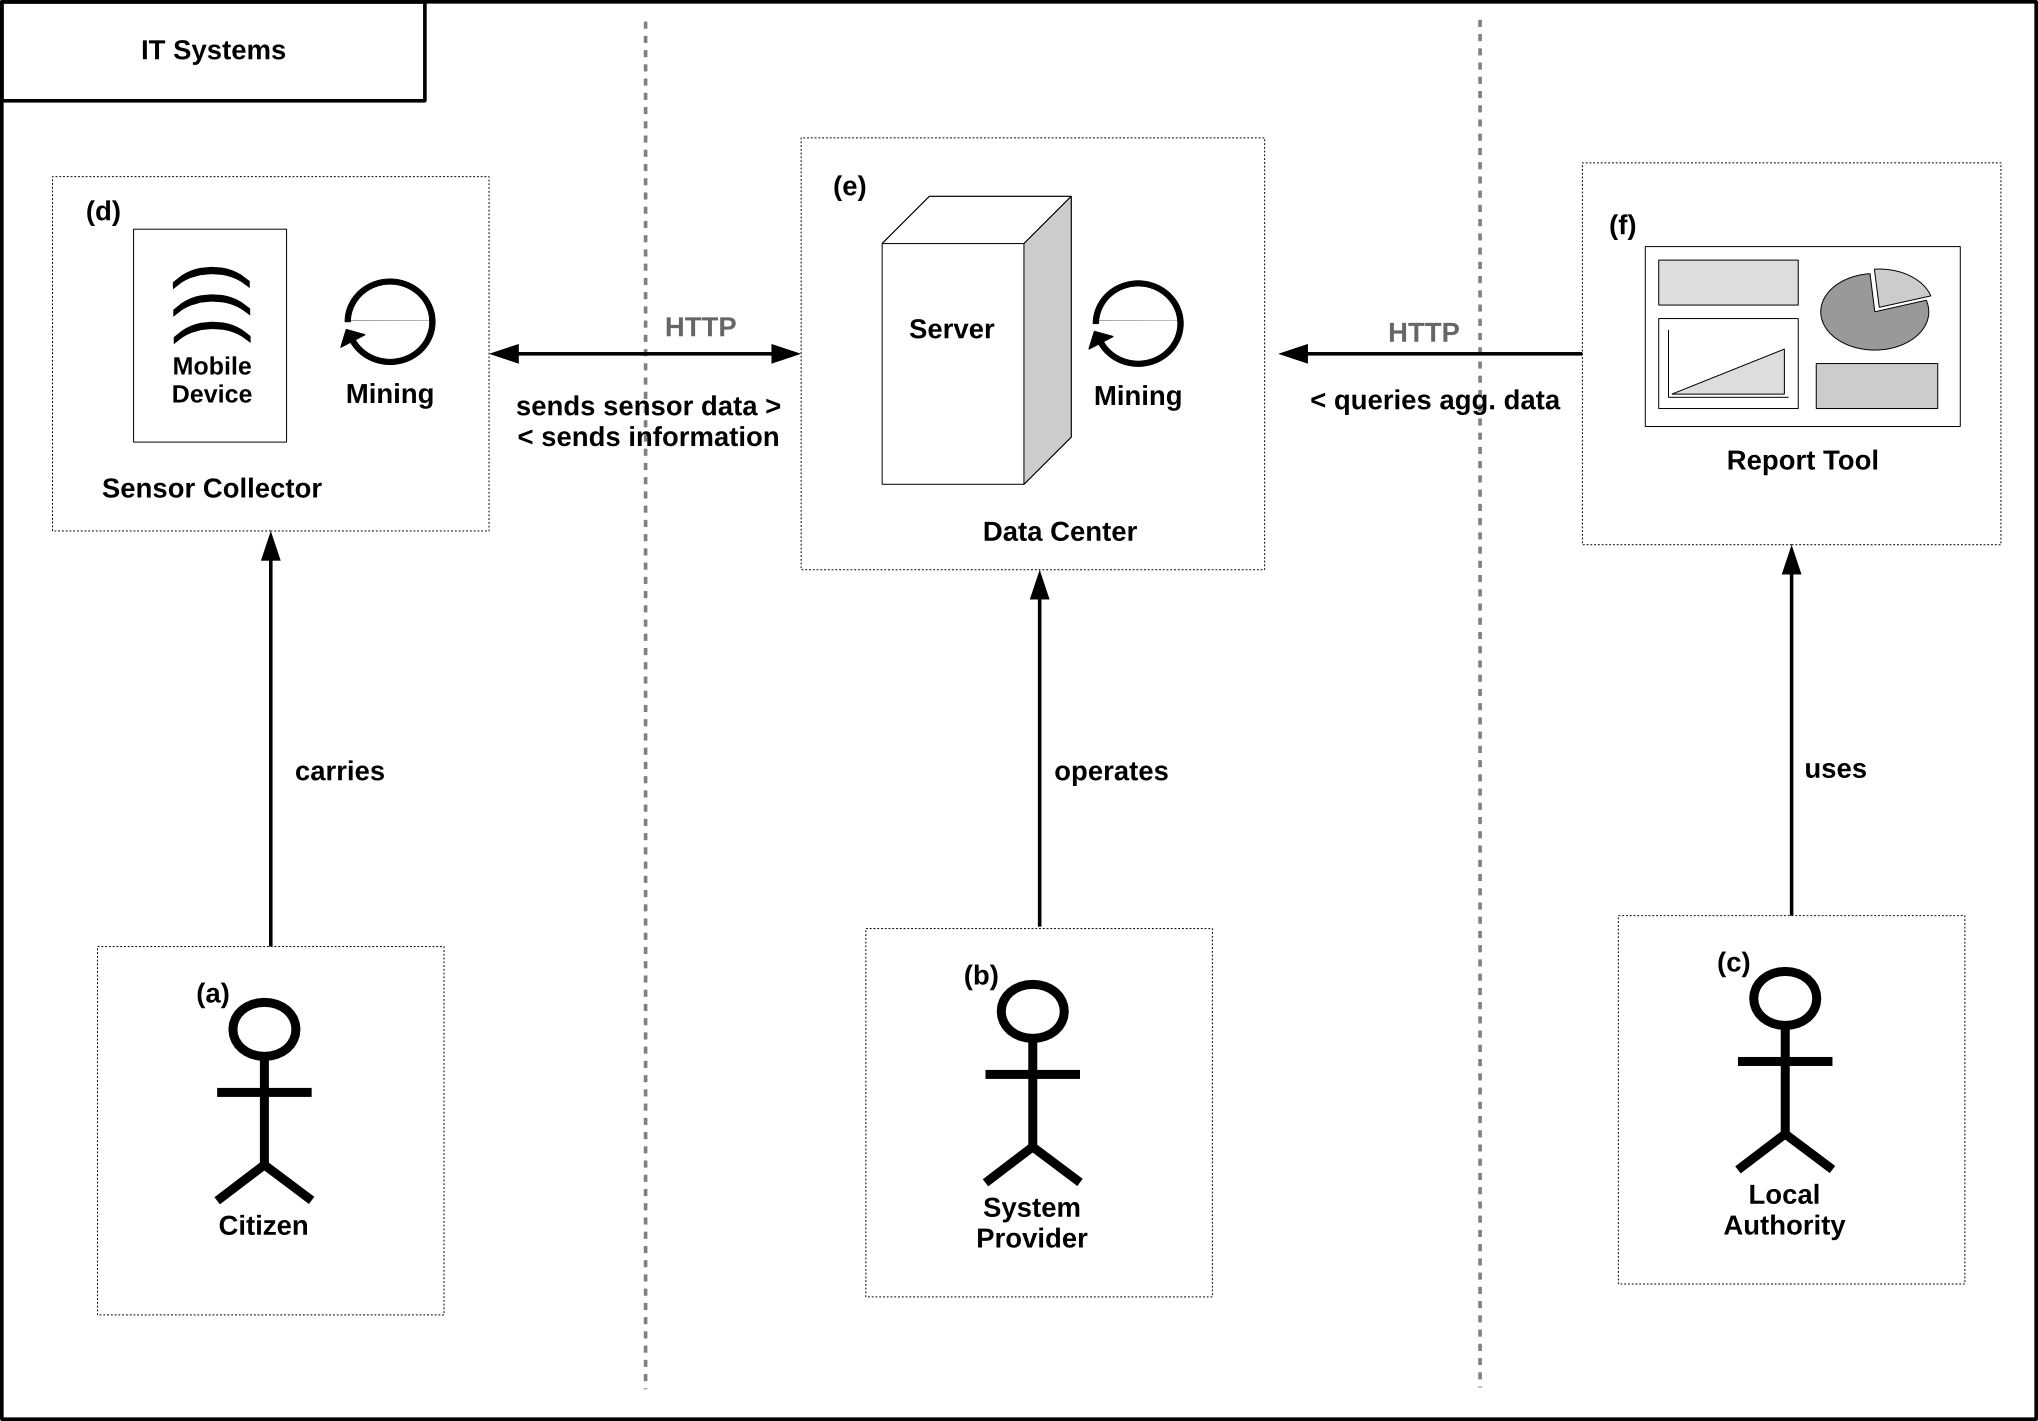
\includegraphics[width=\textwidth]{diagrams/png/it-systems.png}

\begin{flushleft}
\scriptsize
\textbf{Legend:}
\begin{itemize}
\itemsep1pt\parskip0pt\parsep0pt

\item
\textbf{(a) Citizen:} 
User of the L+G client application whose privacy is at stake.

\item
\textbf{(b) System Provider:} Provides technical infrastructure.

\item
\textbf{(c) Local Authority:} Provider of the L+G system.

\item
\textbf{(d) Mobile Device:}
Runs the L+G client application, produces and stores data sensitive to the users privacy.

\item
\textbf{(e) Data Center:} Runs the L+G services, processes and stores user data.

\item
\textbf{(f) Report Tool:} Interface to aggregated user data.

\end{itemize}
\end{flushleft}

\caption{IT Systems}
\label{figure:IT Systems}
\end{figure}


A citizen (a) carries a mobile device running the \emph{sensor collector} (d) application.
The sensor collector application collects sensor data (accelerometer, GPS, GSM, ...) and sends it to the \emph{data center} (c).
The sensor collector can also be able to perform certain data mining operations.
Examples of such data mining operations include human activity recognition,the detection of service lines, detection of characters and faces from images.

The \emph{data center} stores and processes sensor data collected with the sensor collector application.
Again the amount 

Vice versa, it sends beneficial information (traffic jam reports, bus schedule) for \textit{Citizens} to the mobile device.
The \textit{System Provider (b)} provides and operates technical infrastructure like the \textit{Data Center} and the \textit{Report Tool (f)}.
The \textit{Report Tool} queries the \textit{Data Center} for aggregated data to visualize in form of charts and other means suitable to help understanding of monitored \textit{Citizens}. 
\textit{Local Authorities (c)} use the \textit{Report Tool} to get information in order to understand citizen movement and improve public services. 

In such systems, the most valuable information is not the raw sensor data, the beneficial information for \textit{Local Authorities} is produced via \textit{Data Mining} (Human Activity Recognition: detect running, walking, standing, ...). 
Usually, \textit{Data Mining} is heavily conducted within the \textit{Data Center}, but simpler mining processes can also be conducted on mobile devices.



\subsubsection{Actors}
\label{subsubsection:humans}

This section outlines the human actors previously introduced within the IT system architecture (\ref{subsubsection:it-systems}).
It is described which individual interests they have invested in monitoring systems comparable to the Live+Gov system. 
Also the additional actor \textit{Criminal} is introduced as an possible obstacle.

\textbf{Citizen:} 
Citizens are persons who take part in the monitoring system as the monitored subjects.
They offer their privacy sensitive data, because by participating they expect a higher level of comfort in their lives through the offered services in return.
E.g. they will have access to real time bus schedules and traffic jam reports, localized social networking or they generally benefit from public improvement by Local Authorities.

However, they have a legal right to privacy and are interested in having that privacy respected by others.
For example, all humans have a natural interest in physical wellbeing and personal health. 
If someone monitors their immediate location (GPS) or frequently used routes (stalking), people with access to that information could attack and harm citizens.

In general, citizens are not interested in having information about them exploited by others. 
This includes just annoying spam, where their technical identity is used to send unwanted commercials.
But it also includes more severe phishing attacks, which try to rob citizens of their TAN numbers and disrespect their financial interests.

Such financial interests of monitored citizens, the interest in not losing / gaining money, could be disrespected on an even larger scale.
Collected data could be used for scoring and analysis, which may affect the pricing of policies or credits, if sold to insurances or banks.

So citizens have an inherent interest in transparency and disclosure of who uses their data for which purposes, as it may affect their physical and financial wellbeing.

In short, Citizens are interested in ...
\begin{itemize}
\item ... confidential use of privacy sensitive data
\item ... legitimate use of privacy sensitive data
\item ... proportional use of privacy sensitive data
\item ... successful use of privacy sensitive data
\end{itemize}

\textbf{Criminal:}
Criminals are persons who do not have legal access to the IT systems of a proposed monitoring system.
Usually, monetary interests lead their activities.
For example they want to obtain access to critical systems to steal sensitive data or to get the system under their control.
Controlled systems could be leased as part of a bot net. 
Stolen data could simply be sold as is or used for illegitimate purposes, e.g. spam or phishing attacks - or excessive data mining.  

Because Local Authorities are involved in the general outline of a public monitoring system, the possibility for politically motivated attacks cannot be ignored. 
Criminals could want to harm or destroy the systems in order to damage the reputation of Local Authorities (politicians or other officials) or to make a political statement of their own, e.g. "Stop Surveillance!".

Another possible motivation for criminal activities could be social appreciation.
A hacker could attack critical infrastructure just to prove his skills.

In short, Criminals are interested in ...
\begin{itemize}
\item ... financial profit
\item ... high social standing
\item ... political power
\end{itemize}

\textbf{System Provider:}
System Providers provide and operate the technical infrastructure (hardware and software) of the proposed monitoring system.
They are normal companies which offer to provide a service, so different roles of employees are involved:
 an administrator, who maintains and operates the running system;
 a programmer/developer, who develops the system;
 a support manager, who handles customer relations;
 etc.

As companies, they are interested in gaining financial profit.
Among other things, this depends on customer satisfaction, employee happiness and task complexity.
Unsatisfied customers may not want to pay for the service or do not continue the business relation.
Moreover, unsatisfied customers can create a bad reputation, which affects the market for future customers.

Customer satisfaction is connected with the quality of the offered product or service.
This quality depends on the happiness of employees. 
Employees have a claim to professional excellence.
They want to deliver a good job within their means.
If employees cannot satisfy their demand for professional excellence, they might get discontent and deliver poor work.
Moreover, unhappy employees can produce higher costs through sick days.
Ill employees stay on payroll, but stress the project schedule by splitting the workload on fewer heads.
The worst case scenario could be, that a discontent employee gets angry and steals data or harms the running systems.

At last, the financial success of System Providers depends on the task complexity.
The complexity of a task has to be in reasonable bounds, so that System Providers can complete it within time, with a satisfying quality.
If a task has a higher complexity than expected, financial loss is almost determined.
Either System Providers need to hire additional competence to meet schedule and requirements.
Or System Providers they stress the time-line, which also results in a higher man-hour salary ratio and additionally endangers customer satisfaction.
Ultimately, high task complexities can affect employee happiness, if employees cannot complete it within their claim to professional excellence.  

In short, System Providers are interested in ...
\begin{itemize}
\item ... financial profit
\item ... good working conditions
\item ... professional excellence
\item ... reasonable complexity
\end{itemize}


\textbf{Local Authority:} 
Local Authorities are public offices (ministry, agency, department, ...) or other external public service providers which act as direct customers of Service Providers.
They order a proposed monitoring and mining system specialized for their needs. 
For example a low level department, like departments for public mobility, orders a monitoring and mining system to better understand and improve urban traffic flow.

Such systems are heavy investments, so naturally Local Authorities are interested in a profitable return.
However, the return of investment is not directly of financial nature.
Like Service Providers their financial gain depends on customer satisfaction. 
Customers for Local Authorities are either citizens, who use their services, or politicians, who order their services.
The happiness of both sides is interdependent. 
Citizens are happy customers if the services, e.g. public mobility, work well. 
If citizens are happy, it is more likely that politicians gain reputation, as they organize the public services through Local Authorities.

One way of achieving these business objectives is by utilizing business intelligence. 
A proposed monitoring and mining system can provide such intelligence.
For public mobility services it can provide traffic jam detection to maximize traffic flow.
Or it can provide user profiling to maximize (targeted) publicity.

Additionally, since Local Authorities act like corporations comparable to Service Providers, they are also interested in good working conditions.
As discontent employees may harm the system by disclosure of business intelligence.

In short, Local Authorities are interested in ...
\begin{itemize}
\item ... business intelligence
\item ... political reputation
\item ... good working conditions
\end{itemize}


\subsubsection{Conflicts of Interests}
\label{subsubsection:Conflicts of Interests}
This section outlines the Conflicts of Interests (Figure \ref{figure:Live+Gov Conflicts of Interests}) between the actors of the proposed IT system architecture. 
The individual interests of all actors is already described in the previous section and are not elaborated any further.
The emphasis here is put on prominent existing conflicts, because they provide a foundation for vulnerabilities and subsequent threats.

\begin{figure}
\centering
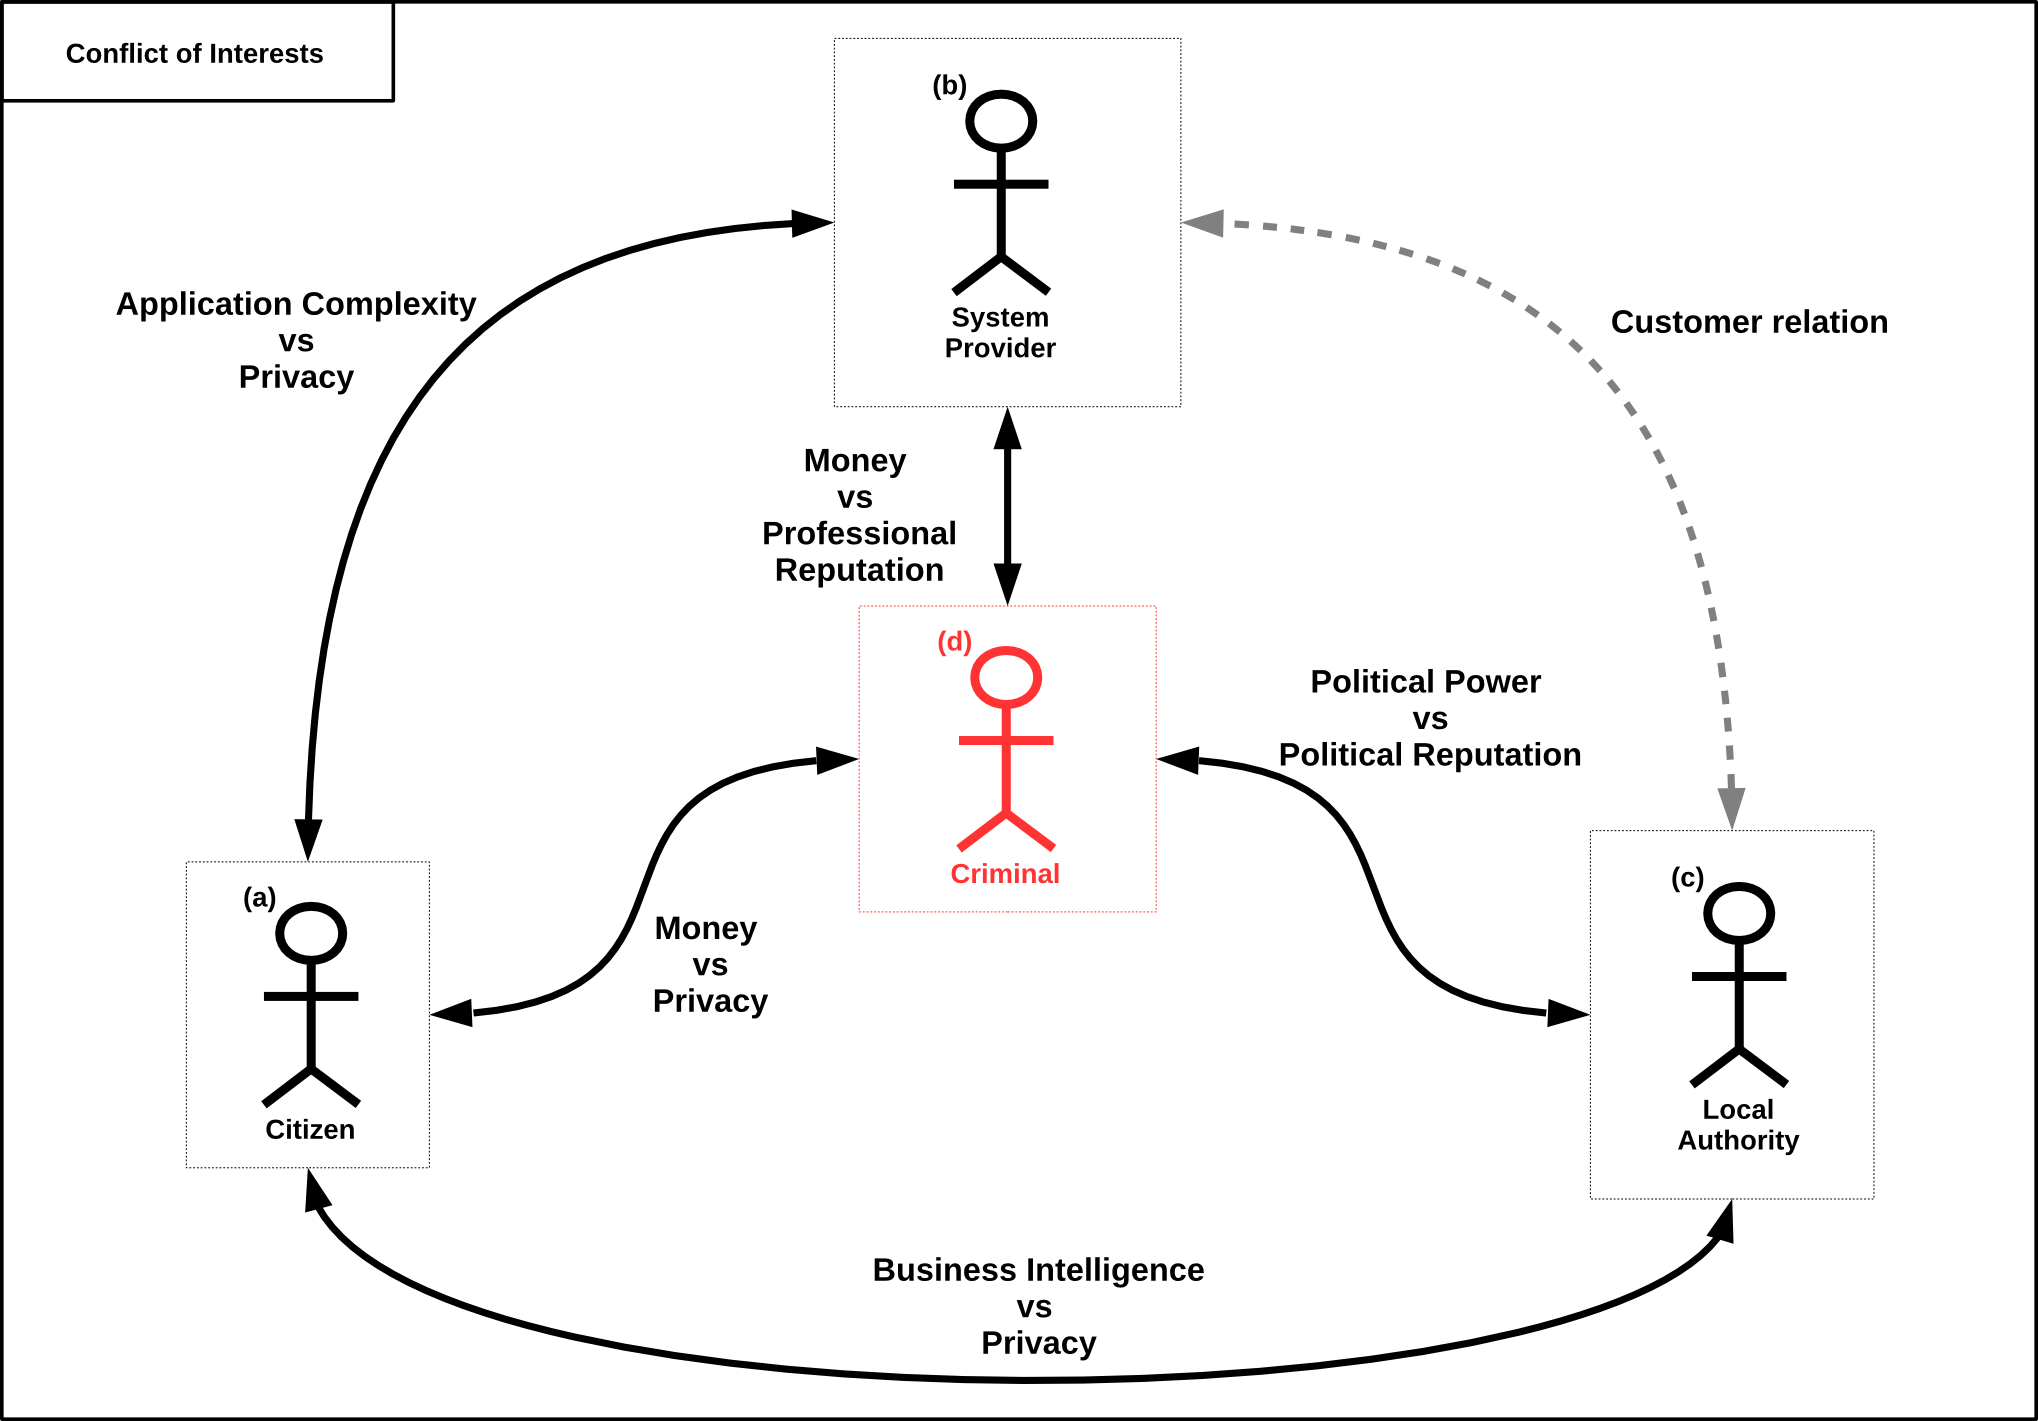
\includegraphics[width=\textwidth]{diagrams/png/conflict-of-interests.png}
\caption{Live+Gov Conflicts of Interests}
\label{figure:Live+Gov Conflicts of Interests}
\end{figure}



\textbf{System Complexity vs Privacy:}
System Providers offer a service to Local Authorities, which is to provide and maintain a monitoring and mining system, e.g. for public mobility.
This system shall produce business intelligence, so that Local Authorities can improve their public services.
This task in it self has a high technical complexity and is the sole asset with financial return for System Providers.
However, this task operates on privacy sensitive data provided by monitored Citizens.
In order to ensure their privacy, System Provider would have to implement additional mechanisms, which allow Citizens to exercise control of their data.
But this will eventually raise the complexity of the monitoring and mining system.


\textbf{Business Intelligence vs Privacy:}
Local Authorities order a monitoring and mining system from System Providers, which allows them to produce business intelligence for public services.
The system is a heavy investment for Local Authorities, so they are interested in as much intelligence as possible to achieve a profitable return.
But the intelligence is the result of data mining conducted on privacy sensitive data of monitored Citizens.
They are interested in the successful usage of their data, in a sense that they are also benefactors, e.g. improvement of public mobility.
However, the main interest of Citizens lies in maintaining control over their data.
In order do that, they need disclosure of the exact purposes their data is used for, so they can select which data to share.
These purposes cannot be (secretly) exceeded.


\textbf{Money vs Privacy:}
Criminals can gain financial profit from stealing privacy sensitive data.
For example by selling raw contact information to advertisers or by selling mined data to scoring services.
In such cases, Citizens lose complete control over their data.


\textbf{Money vs Professional Reputation:}
Criminals have various business models as optional foundation for attacks on System Providers.
For instance, they can try to invade the infrastructure for e-espionage reasons, to get control over servers to create a bot-net or to steal user data.
All these approaches are motivated by financial interests.
Gathered information can be sold, zombie servers can be leased.
A successful attack proves the technical competence of System Providers wrong and subsequently harms their professional reputation.
This can lead to a loss of future customers or a decrease of stock price for registered companies.
Eventually the financial interests of System Providers are endangered.


\textbf{Political Power vs Political Reputation:}
Besides monetary reasons, Criminals can be motivated by political reasons to attack the monitoring and mining system.
Criminals can break the system to make a political statement of their own, e.g. "Stop Surveillance!".
Or they can steal user data to prove the system insecure.
Both would harm the political reputation of Local Authorities, who endangered the privacy of monitored Citizens.
Criminals would gain political power, because their point of view would seem to be valid.




\subsubsection{Vulnerabilities}
This section outlines the vulnerabilities (Figure \ref{figure:Live+Gov Vulnerabilities}) of the proposed monitoring and mining system.
Note that vulnerabilities are not necessarily of technical nature.
The weaknesses of IT systems are often created due to misuse or misconfiguration of the various components by one or more actors.

\begin{figure}
\centering
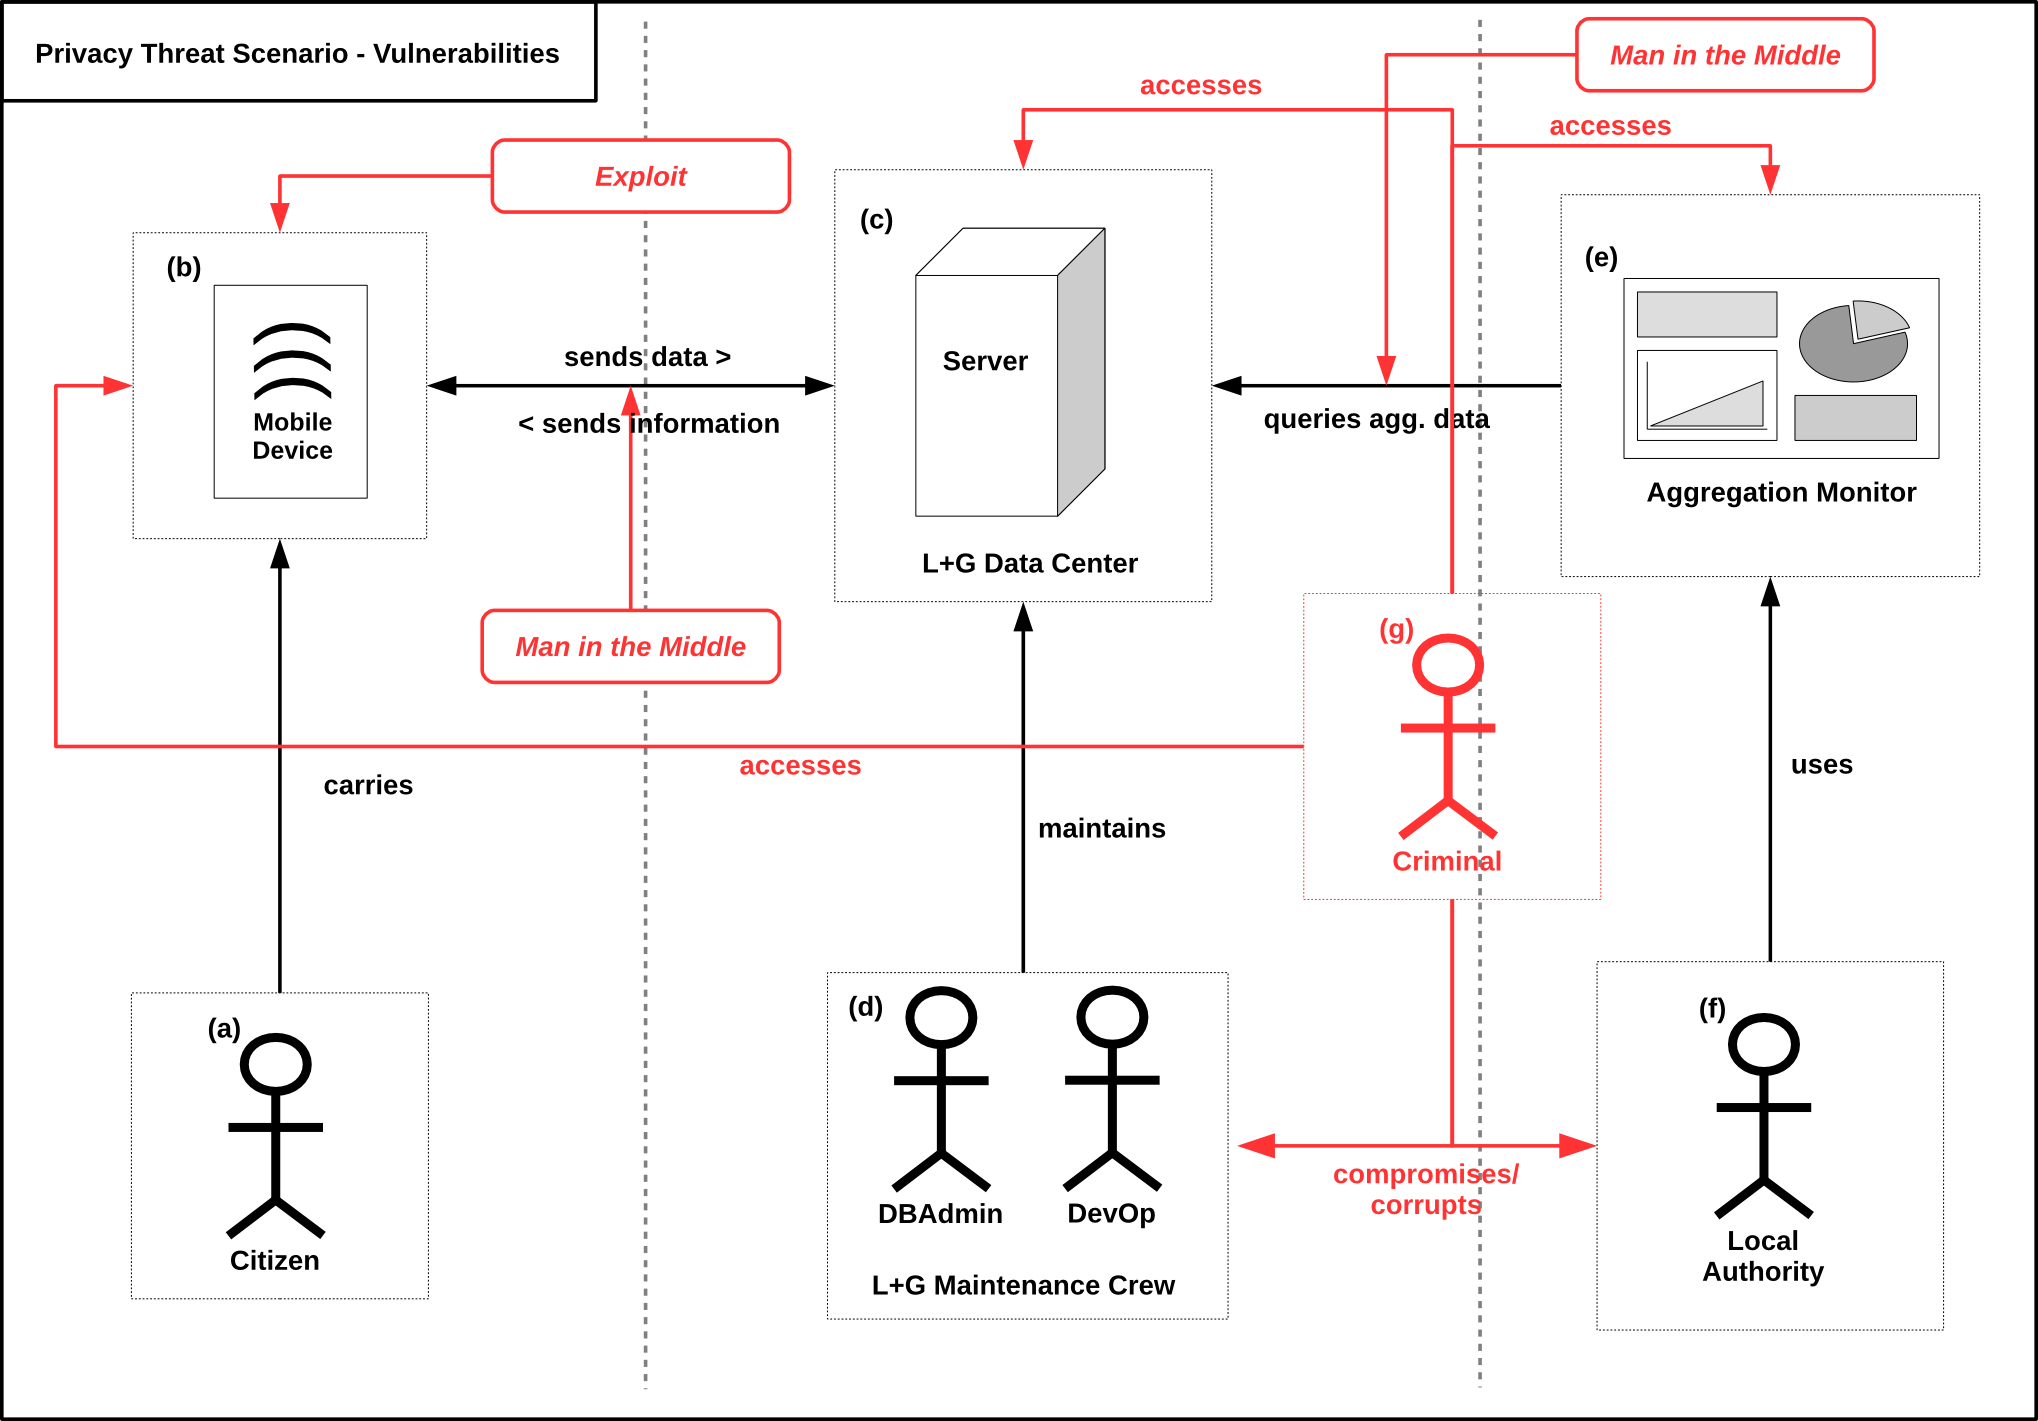
\includegraphics{diagrams/png/scenario-vulnerabilities.png}

\begin{flushleft}
\scriptsize
\textbf{Legend:}

\begin{itemize}
\itemsep1pt\parskip0pt\parsep0pt
\item
  \textbf{(a) Citizen:} User of the L+G client application whose privacy
  is at stake.
\item
  \textbf{(b) Mobile Device:} Runs the L+G client application, produces
  and stores data sensitive to the users privacy.
\item
  \textbf{(c) L+G Data Center:} Runs the L+G services, proccesses and
  stores user data.
\item
  \textbf{(d) L+G Maintenance Crew:} Technical staff with access to
  critical infrastructure.
\item
  \textbf{(e) Aggregation Monitor:} Interface to aggregated user data.
\item
  \textbf{(f) Local Authority:} Provider of the L+G system.
\item
  \textbf{(g) Criminal:} Threatens the L+G system and Citizen privacy.
\end{itemize}
\end{flushleft}

\caption{Live+Gov Vulnerabilities}
\label{figure:Live+Gov Vulnerabilities}
\end{figure}


\textbf{Unencrypted Data Transmission:}
The proposed monitoring and mining system uses HTTP to exchange data between the Sensor Collector, the Data Center and the Report Tool.
Per default, HTTP is a clear text protocol.
This means, one can intercept the connection and read all sensitive information, which is send between the components.
That is: passwords, raw sensor data and data mining results

\textbf{Inadequate Access Rules:}
The proposed IT system infrastructure has various accesses to privacy sensitive data.
System Provider staff has access to Data Center hardware and software like databases, web-servers and other inspection tools.
Local Authority staff has access to the Report Tool.
This all enables staff members to have potential access to privacy sensitive information.
Those accesses have to be secured against unauthorized third parties, e.g. Criminals.
Moreover, we need to ensure that no single person has to many access rights.
For example, a system administrator should not be able to secretly download the whole database on a flash-drive.

\textbf{Insufficiently Secured Infrastructure:}
The proposed monitoring system consists of many hardware and software components, each with its own concrete weaknesses.
For instance, operating systems can be outdated or not subject to frequent updates or virus scans.
Web-applications can be carelessly implemented and not protected against SQL-Injections or Cross-Site-Scripting attacks.
Databases can be ill-configured, so that access from outside the system is possible.
All those weak points can be subject to various known exploit techniques.

\textbf{Unaware Monitoring Subjects:}
We define privacy as one's ability to control information about oneself. 
In order to do that, monitored subjects need to know, that they are monitored, who monitors them, what information is recorded and for what purposes.
Subjects who are not aware of these things cannot effectively preserve control and thus lose their privacy.


\subsection{Step 2. Potential Analysis}

\subsubsection{Threats}
\begin{figure}
\centering
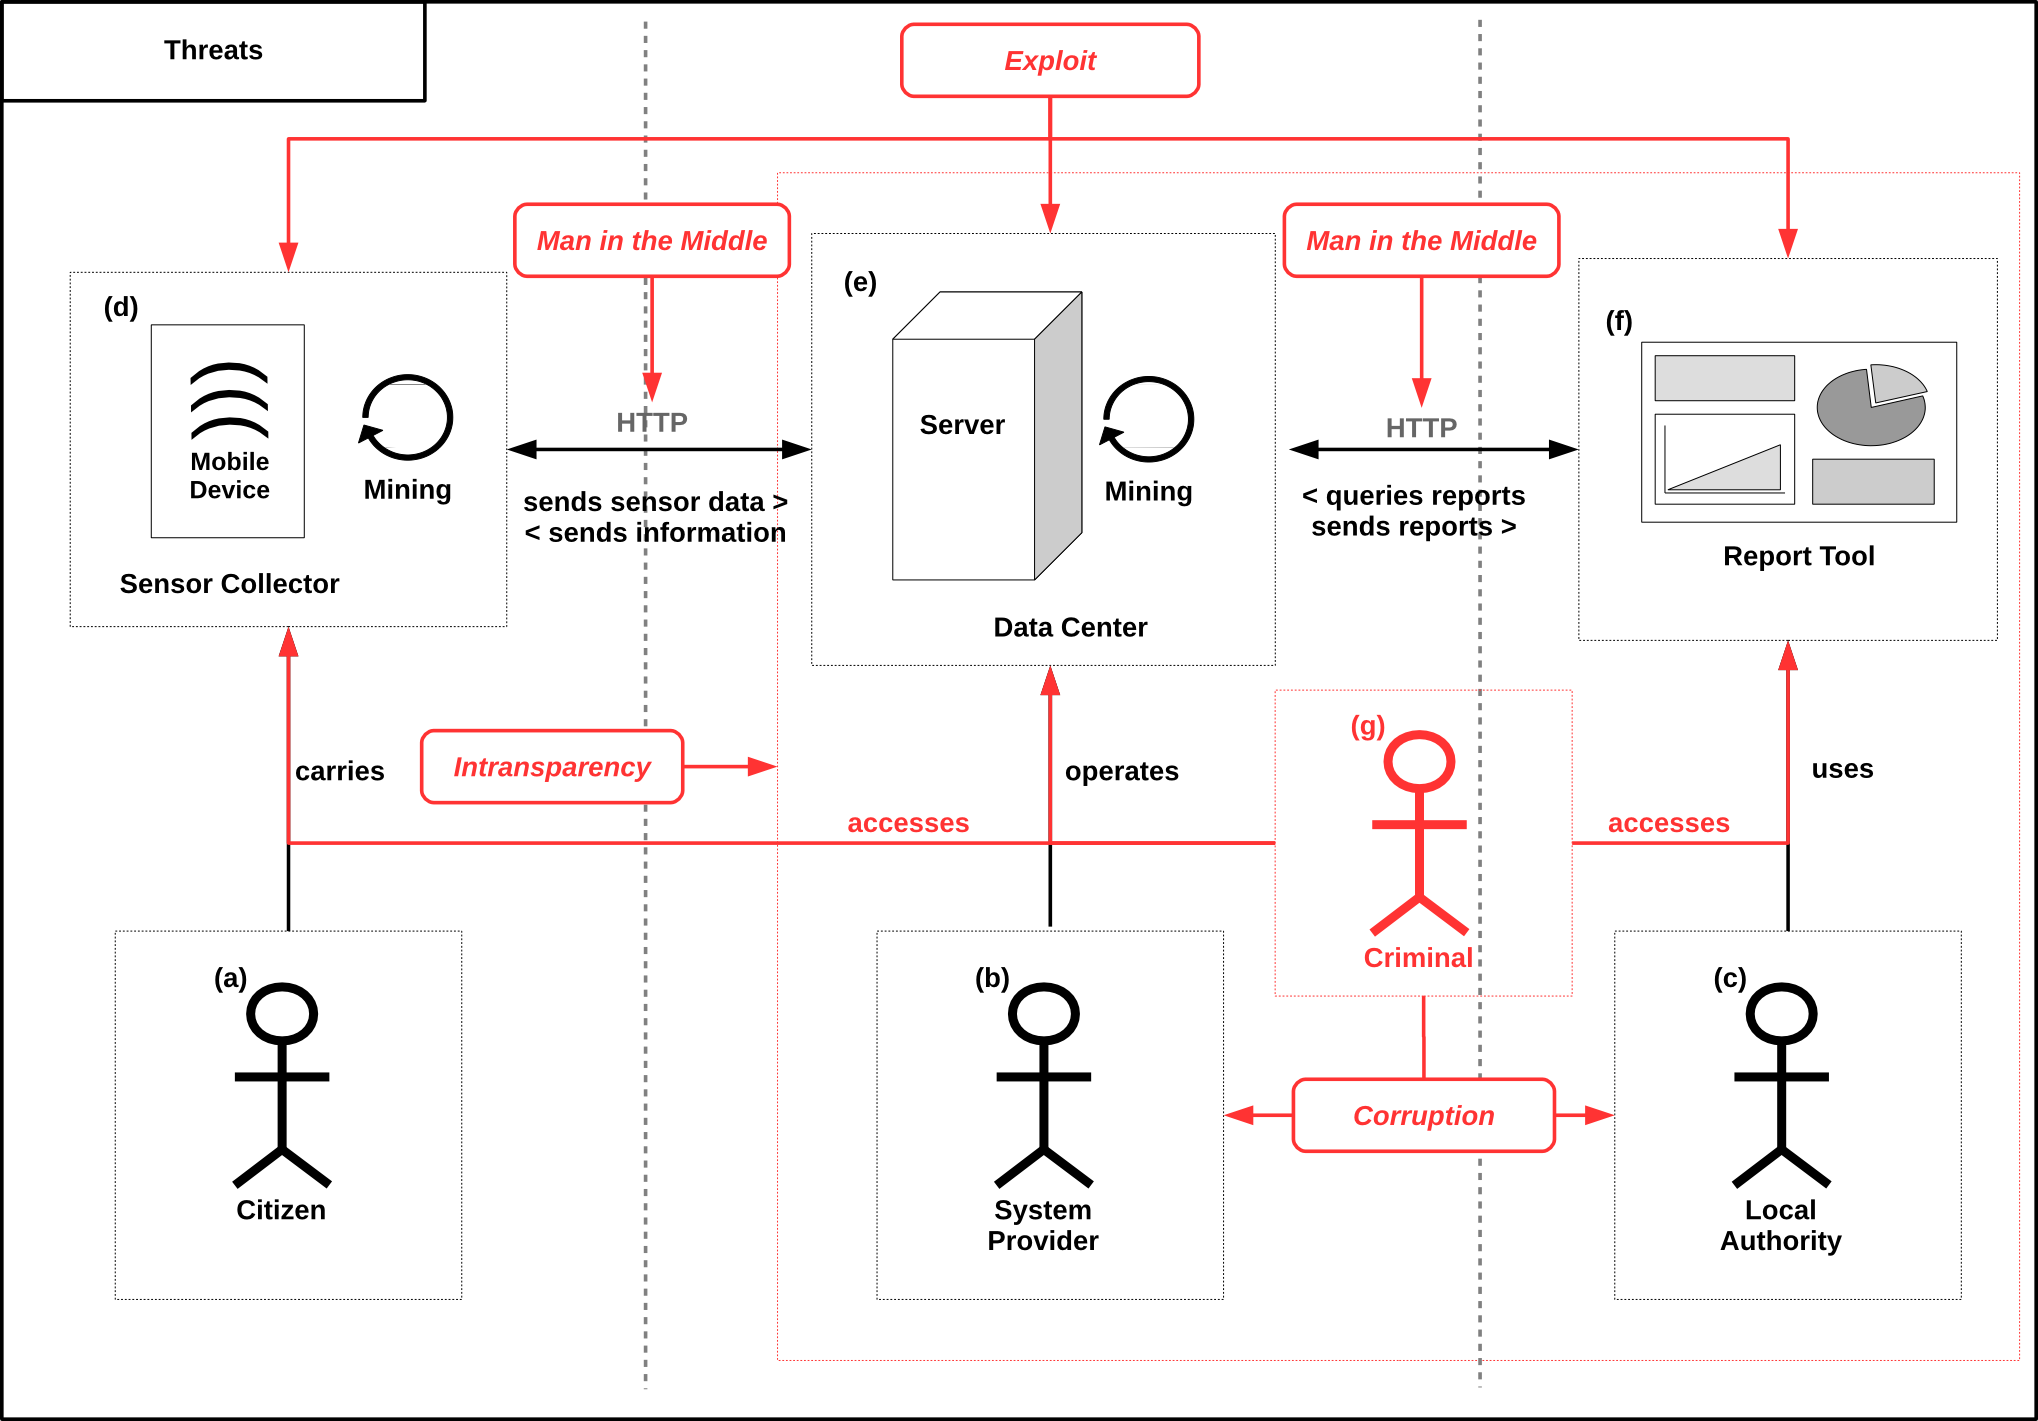
\includegraphics[width=\textwidth]{diagrams/png/threats.png}

%\begin{flushleft}
%\scriptsize
%\textbf{Legend:}
%
%\begin{itemize}
%\itemsep1pt\parskip0pt\parsep0pt
%\item
%  \textbf{(a) Citizen:} User of the L+G client application whose privacy
%  is at stake.
%\item
%  \textbf{(b) Mobile Device:} Runs the L+G client application, produces
%  and stores data sensitive to the users privacy.
%\item
%  \textbf{(c) L+G Data Center:} Runs the L+G services, proccesses and
%  stores user data.
%\item
%  \textbf{(d) L+G Maintenance Crew:} Technical staff with access to
%  critical infrastructure.
%\item
%  \textbf{(e) Aggregation Monitor:} Interface to aggregated user data.
%\item
%  \textbf{(f) Local Authority:} Provider of the L+G system.
%\item
%  \textbf{(g) Criminal:} Threatens the L+G system and Citizen privacy.
%\end{itemize}
%\end{flushleft}

\caption{Live+Gov Threats}
\label{figure:Live+Gov Threats}
\end{figure}

% =================================================
% Threat Table Macros

% Const Column Width
\newcommand{\ThreatTableColWidth}{5cm}

% Const Header Row Height
\newcommand{\ThreatTableHeaderRowHeight}{0.5cm}

% Const Content Row Height
\newcommand{\ThreatTableContentRowHeight}{1cm}

% Define Header Cell Makro
\newcommand{\ThreatTableHeaderCell}[1]{
\begin{minipage}[t][\ThreatTableHeaderRowHeight][c]{\ThreatTableColWidth}
\centering
\scriptsize
\textbf{#1}
\end{minipage}
}

% Define Content Cell Makro
\newcommand{\ThreatTableContentCell}[1]{
\begin{minipage}[t][][c]{\ThreatTableColWidth}
\begin{flushleft}
\tiny
#1
\newline
\end{flushleft}
\end{minipage}
}

% Define Header Row Makro
\newcommand{\ThreatTableHeaderRow}[4]{
\ThreatTableHeaderCell{#1}
&\ThreatTableHeaderCell{#2}
&\ThreatTableHeaderCell{#3}
&\ThreatTableHeaderCell{#4}
\\ \hline
}

% Define Content Row Makro
\newcommand{\ThreatTableContentRow}[4]{
\ThreatTableContentCell{#1}
&\ThreatTableContentCell{#2}
&\ThreatTableContentCell{#3}
&\ThreatTableContentCell{#4}
\\ \hline
}

%  Define Threat Table Environment
\newenvironment{ThreatTable}
{
\begin{tabular}{|c|c|c|c|}
\hline
\ThreatTableHeaderRow
{Description}
{Conflict of Interest}
{Vulnerabilites}
{Assets (Privacy Types)}
}
{\end{tabular}}


% =================================================
% Threat Table Content

\begin{landscape}
\begin{figure}
\centering
\begin{ThreatTable}

\ThreatTableContentRow
{\textbf{(Zero Day) Exploits}
\\A criminal uses (Zero Day) Exploits to obtain access to hardware or software which stores or processes
privacy sensitive data in order to get that data.}
{Criminals want to obtain access or data for personal profit, i.e. by (re-)selling the data or  by processing it themselves. 
However, criminals may have no financial interest, they could also gain personal (ego) profit by testing proof-of-concept attacks.
\\\textbf{Criminal vs Citizen}
\\Citizens only allowed Local Authorities to use their data. They want their data to be secret to others. (Additionally, citizens are
also interested in a working system, which they payed for via taxes.)
\\\textbf{Criminal vs Local Authorities}
\\Local Authorities have capital and reputation invested in a working system. Successful attacks undermine both.
\\\textbf{Criminal vs Maintenance Staff}
\\Staff members have a professional ethos and a duty to provide working systems. Successful attacks offend the former and obstruct the latter.
\\Staff member employed by L+G or contractor. The Business operation is thretened by loss of confidential data.
}
{Unsecured Hardware- or Software-Interfaces}
{\textbf{Explicit:} 1,4,6,7}

\ThreatTableContentRow
{\textbf{Man in the Middle} 
\\A criminal intercepts communication between mobile device and server or between server and application.}
{\textit{Like Exploits}}
{Unencrypted hardware or software communication}
{\textbf{Explicit:} 1,4,6,7}

\ThreatTableContentRow
{\textbf{Corrupt Employees} 
\\ An employee abuses his database access to obtain private citizen data in order to sell it to advertisers.}
{\textbf{(Corrupt) Employee vs Citizen} 
\\ Corrupt Employees want to make personal profit by selling citizen data. 
Citizens provide data for public improvement, they don't want their data to be used for other purposes, which
may lead to negative effects for themselves.
Employees in general need easy database access to do their job. But this also means easy access to privacy
sensitive data of citizens. This diametrically opposes the interest of citizens to have such information unknown
to other individuals.}
{Full database access of Employees}
{\textbf{Explicit:} 1,4,6,7}

\ThreatTableContentRow
{\textbf{Corrupt Local Authorities}
\\A member of the Local Authority abuses his access to applications 
to obtain aggregated citizen data in order to use it for illegitimate purposes, e.g. selling it.}
{\textbf{(Corrupt) Local Authority Member vs Citizen}
\\\textit{Like Corrupt Employees}}
{Full application access of Local Authorities}
{\textbf{Explicit:} 1,4,6,7}

\ThreatTableContentRow
{\textbf{Careless Citizen}
\\A careless citizen allows others (Criminals) to have unrestricted access to his mobile device. 
Hence, he creates to possibility to install spy-ware or have the device destroyed.}
{\textbf{Criminal vs Citizen}
\\Criminals want to have access to mobile devices to obtain private data of citizens in order to 
gain personal profit - or to simply render the device useless. On the other hand, citizens have a 
natural interest in keeping personal data secret in order to prevent financial loss or because having
sensitive information accessible to others violates their privacy.}
{Insufficient access rules for mobile devices}
{\textbf{Explicit:} 1,4,6,7}

\ThreatTableContentRow
{\textbf{Intransparent Data Mining}
\\Local Authorities or System Providers use their technical knowledge, data mining capabilities and 
additional data sources to obtain/create more information about citizens.}
{\textbf{Citizen vs Local Authority or System Provider}
\\Citizens only agreed to share certain sensitive data with Local Authorities and System Providers to help society.
They are not interested in negative effects as a result of such a good willing act.
However, Local Authorities and System Providers have an interest to maximize the profit of their investments.
Local Authorities could (secretly) use mined data for security or health care issues. System Providers could
(secretly) sell mined data to illegitimate customers, e.g. the SCHUFA. This could lead to repressive behaviour of law
enforcement or negative scores.}
{Unaware Citizens}
{1,2,3,4,5,6,7}

\end{ThreatTable}

{\scriptsize (\textbf{Note for Meeting:} I think we need discrete (numbered) lists of interests for each actor in the \textit{Humans} section.)}

\caption{Threat Table}
\end{figure}
\end{landscape}


%\begin{itemize}
%
%\item
%  \textbf{Unauthorized access to privacy sensitive data}, caused by
%  \begin{itemize}
%  \item
%    \textbf{Excessive Data Mining} Linking sensor data provided by
%    citizens with additional sources can produce more privacy sensitive
%    data.
%  \item
%    \textbf{Corrupt Local Authorities} Local Authorities have certain data
%    access, they could hand over this access for monetary reasons.
%  \item
%    \textbf{Corrupt/Unhappy Staff} Staff members also have a certain data
%    access and they also could hand over this access for monetary reasons
%    or as a form of payback for unfair treatment.
%  \item
%    \textbf{Competent Attackers} Competent Attackers are always a threat
%    for IT-systems. Normaly they have monetary reasons to exploit a
%    system, but there is also a possibility for proof-of-concept like
%    attacks.
%  \end{itemize}
%\end{itemize}
%
%
\paragraph{Sensor Privacy Matrix (Figure \ref{figure:Live+Gov Sensor-Privacy Matrix})}

%\includegraphics{../diagrams/png/sensor-privacy-matrix.png}
\begin{figure}
\centering
\includegraphics[width=\textwidth]{diagrams/png/sensor-privacy-matrix.png}


\begin{flushleft}
\scriptsize
\textbf{Legend:}
\begin{itemize}
\itemsep1pt\parskip0pt\parsep0pt
\item
  The x-axis lists the 7 Types of Privacy according to Friedewald et al.
\item
  The y-axis lists all mobile sensors currently used by the Live+Gov
  procject.
\item
  The big black bullet point dentotes that there is a \textbf{direct}
  violoation of a privacy type from a sensor
\end{itemize}
\end{flushleft}

\caption{Live+Gov Sensor-Privacy Matrix}
\label{figure:Live+Gov Sensor-Privacy Matrix}
\end{figure}


\subparagraph{Privacy of The Person}

The \textbf{Privacy of The Person} is generally concerned with one could
best understand as \emph{Biometric Privacy}. Friedewald et al. paraphrase
it as \emph{``[...] the right to keep body functions and body
characteristics [...] private''}. \textbf{Accelerometer},
\textbf{Rotation Vector} and \textbf{Gyroscope} measure the physical
movement of the mobile device on all three axes. If the mobile device
is carried \emph{``normally''} its safe to say that those sensors also
measure the moments of its carrier. So his privacy is infringed
regarding biometric behaviour, as it is captured automatically.
(\textbf{Note:} This is not to be confused with the \textbf{Privacy of
Behaviour and Action} which is used for the social aspects of behaviour
action, e.g.~praying, sexual habits or political activities.)

\subparagraph{Privacy of Data and Image}

The \textbf{Privacy of Data and Image} demands, that
\emph{``individual's data is not automatically available to other
individuals''}. This type of privacy is trivially threatened because
here sensor data is individual data, a priori. So every sensor violates
the privacy of data and image, as data is transported into a foreign
system where operators have access to it.

\subparagraph{Privacy of Location and Space}

According to Friedewald et al., the \textbf{Privacy of Location and
Space} is concerned with one's \emph{``right to move about in public or
semi-public space without being identified, tracked or monitored.''}.
This is the location aspect of this type. The space aspect is concerned
with one's \emph{``right to solitude''}, which generally includes one's
right to an inviolate home and other private spaces. Obviously the
\textbf{GPS} and \textbf{GSM} sensors violate such right about not being
tracked, because they reveal the position of the mobile device and its
carrier. The \textbf{GSM} sensor gives the exact cell, the mobile device
has registered with at the current moment. The \textbf{GPS} sensor gives
the current longitude and latitude, the current global position of the
mobile device and its carrier, although there is some artificial
inaccuracy within civil use.

The \textbf{WLAN} and \textbf{Bluetooth} sensors record lists of the
currently available local wireless networks and bluetooth clients. If
such are known stationary entities, those sensors are considered as
dangerous as the \textbf{GSM} sensor for the carriers locational
privacy.

The \textbf{Magnetic field} sensor is not regarded very dangerous to the
carrier's privacy, because it does not allow very precise localization.
But it can limit the possibilities for the global position of the mobile
device. Here, it is just named for completeness sake.

\subparagraph{Privacy of Associtation}

The \textbf{Privacy of Association} sates that everyone has the
\emph{``right to associate with whomever they wish, without being
monitored [automatically without reasonable suspicion]''}. This
includes individuals and organizations. \textbf{WLAN} and
\textbf{Bluetooth} sensors provide the ability to monitor such
associations if their lists contain known entities. If one frequently
connects with an organizational wireless network, e.g.~an university
network, an association can be deduced (student or staff). The same goes
for the \textbf{Bluetooth} sensor, if it is stationary. Additionally, if
the recorded bluetooth clients are mobile, it is more or less possible
to deduce association with the technical identity of (yet) anonymous
individuals.

Additionally, the \textbf{GSM} sensor could provide the association with
the GSM operator (\textbf{NEEDS TO BE VERIFIED!}).

%\paragraph{Excessive Data Mining}
%
%\subparagraph{1 Privacy of the Person private''} \cite{1}. Here we are
%concerned wi the personal physiological and psychological p and  This privacy is threat...f \textbf{body characteristics}weight, height,, dna,\ldots) or
%depression emph therapists or other doctors) \textbf{can beevealed orii and emph+Gov project collects sensor data from mobile devices
%(accellerometer, location, \ldots). By a...g \emph{human activityecognition (emph)} techniques we could detect certain movement patterns
%we know the position with of indiviual citizens with a sufficientccurancy, and the Live+Gov project is only applied to a destinct urban
%area. So we could link HAR data with the yellow pages, filter for
%medical specialists and limit the possibilities of pathologic
%conditions. But even without HAR data we could determine a likelihood
%for certain conplaints. Frequent vistits to the dentist does not imply
%healthy teeth.

%\subparagraph{2 Privacy of Behaviour and Action}
%
%\emph{``This type is also concerned with the `protection against
%disclosure of personal matters' through behaviour''}
%\cite{1}. This type is concered with religous
%practices, sexaul habits, political activities, etc. revealed through
%observation. For the Live+Gov project this type is related to t is recirded by default and by linking it to maps a and li phone books those *``personal matters*" could be
%disclosed by frequently visited places (c...s, brothels, party headuaters, \emph).
%
%communications' either electronic or face-to-face'' \cite{1}. This type
%is threatened if we intrude the secrecy of correspondence, posts and
%telecommunications, personal direct communication or right to free
%discussion without third parties listening. The Live+Giv project only
%could threaten this type by using mobile client application as trojan
%horse, collecting any communication data (chat, sms, microphone).
%
%\subparagraph{4 Privacy of Data and Image}
%
%\emph{``This type is concerned with `making sure that individuals's data
%is not automatically available to other individuals and
%organisations'\,''} \cite{1}. This is
%Informational Privacy in an intuitive sense regarding data like:
%
%\begin{itemize}
%
%\item
%  Phone Number
%\item
%  IP Address
%\item
%  Public-administrative Data (Date of Birth, population register)
%\item
%  Data held by organizations, like Banks or Insurance Companies
%\item
%  All data that is stored in online services (Facebook)
%\end{itemize}
%
%The Live+Gov project does not threaten this type directly if we assume a
%secure and closed system. However, this privacy type could be threatened
%by carelessly ignoring known (technical) vulnerabilities regarding data
%security. Additionally we could threaten the Privacy of Data and Image
%indirectly by linking collected data with other sources.
%
%\subparagraph{5 Privacy of Thoughts and Feelings}
%
%\emph{``This type is the right `not to share their thoughts or feelings
%or to have those thoughts or feeling (sic!) revealed'\,''}
%\cite{1}. This means thoughts and emotions must
%not be detected autmatically. Intuitively the Live+Gov system seems
%unable to threaten this type. However, considering the issue component
%of the Urban Maintaince use case, this might reveal information about
%one's thoughts regarding the community in a positive manner. Solely by
%taking part we could assume a caring personality. This threatens one's
%privacy in a rather technical sense, but does not necessarily impose any
%harm.
%
%An other way of threatening this type could be constructed by recording
%one's voice with the phone's microphone and run emotion detecting
%algorithms against this data.
%
%\subparagraph{6 Privacy of Location and Space}
%
%\emph{``This type is the right `to move about in public or semi-public
%space withoug being identified, tracked or monitored'. Additionally this
%type is concerned with the protection of one's home and private places
%(`right to solitude')''} \cite{1}. The location
%dimension of this type is relatively easy to understand: The
%geo-position of citizens cannot be monitored by default. However, by
%actively taking part in the Live+Gov project, the locational privacy of
%citizens is threatened by default because data of the location sensor
%will be collected. The space dimension is more complex, but can be
%simplified with a \emph{``right to solitude''}. This dimension could be
%threatend with the invasion of personal space in any means, i.e.~by
%disrespecting one's right to an inviolate home or by undercutting one's
%comfort zone in an conversation. Live+Gov only utilizes the mobile
%devices of citizens, so we could disrespect the former by activating the
%phone's micropone and start recording.
%
%\subparagraph{7 Privacy of Association}
%
%\emph{``This type is the right `to associate with whomever [one]
%wish, withoug being monitored'.''} \cite{1}. This
%means that one's associations must not be recoreded by default
%independet from any suspicion. Anyhow, it does not mean that this right
%cannot be forfeit given a reasonable suspicion. The Live+Gov project
%could easily threaten this type just by linking locational data with
%yellow pages and a map. Even if an association graph cannot be deducted
%for individual citizens, we could aggregate the data to create an
%association graph for a whole population as the Live+Gov system is
%applied to a restricted urban area.

\subsection{Step 3. Plan Development}

\subsubsection{Security Measures}

\paragraph{The 7 C's of user privacy control (Figure \ref{figure:The Seven Cs of User Privacy Control})}

This is a note on an excerpt from the article \emph{Sociotechnical
Architecture for Online Privacy} \cite{1} called
\textbf{The 7 C's of user privacy control}. Those 7 C's are aspects
which should be covered by measures for implementing user privacy. They
derive from an interpretation of privacy which could be summarized as
\emph{``One's ability to control/seclude information about oneself''}.

%\includegraphics{../diagrams/png/The7Cs.png}
\begin{figure}
\centering
\includegraphics[width=\textwidth]{diagrams/png/The7Cs.png}
\caption{The Seven Cs of User Privacy Control}
\label{figure:The Seven Cs of User Privacy Control}
\end{figure}


\subparagraph{Comprehension}

\emph{``Users should \textbf{understand} ho personal identifiable
information (PII) is handled, who's collecting it and for what purpose,
and who will process the PII and for what purpose. Users are entitled
to know all parties that can access their PII, the limits to processing
transparency, why the PII data is being requested, when the data will
expire (Either from a collection or database), and what happens to it
after that. This category also include legal rights around PII, and the
implications of a contract when one is formed.''}

This C implements transparency regarding user data and user privacy.
Comprehension should answer the following questions:

\begin{itemize}

\item
  \emph{WHO} collects data?
\item
  \emph{WHAT} data will be collected?
\item
  \emph{WHY} will data be collected and processed?
\item
  \emph{HOW} will data be collected and processed?
\item
  \emph{WHEN} will data expire?
\item
  What is allowed?
\item
  What choices ar possible?
\end{itemize}

All in all information of what's happening and why has to made
accessible for users.

\subparagraph{Consciousness \textbf{(critical!)}}

\emph{``Users should \textbf{be aware} of when data collections occurs,
when a contract is being formed between a user and data collector when
their PII is set to expire, who's collecting the data, with whom the
data will be shared, how to subsequently access the PII, and the
purposes for which the data is being collected.''}

This C seems to be critical for privacy protection. Consciousness
complements Comprehension in respect that the latter just states that
hard facts need to be delivered. However, those facts might get hidden
in a terms and conditions section which nobody reads but still accepts
anyway. In order to prevent that Consciousness states that a certain
level of \textbf{Awareness} of those facts needs to be established.

\subparagraph{Choice}

\emph{``Users should \textbf{have choices} regarding data collection
activities in terms of opting in or out, whether or not to provide data,
and how to correct their data.''}

Self explaining. This is the actual control enabled by the 7 C's.

\subparagraph{Consent}

\emph{``Users must first \textbf{consent} (meaning informed, explicit,
unambiguous agreement) to data collection, use, and storage proposals
for any PII. Privacy consent mechanisms should explicitly incorporate
the mechanisms of comprehension, consciousness, limitations, and
choice.''}

This C might be special case of Choice. Before taking part a user should
have the choice whether to join or not (Opt-In).

\subparagraph{Context}

\emph{``Users should \textbf{be able to change privacy preferences}
according to context. Situational or physical context - such as crowded
situations (for example, when at a service desk where several people
can listen in on your exchange when you provide a phone number, or when
you're in an online community chat room) - is different from when you
perform a buy transaction with Amazon.com or in rooms with cameras
(where digitization makes the information permanent and unmistakably
you) and data context (such as the sensitivity of data, for example
health data could dictate different actions on the same PII in different
contexts.''}

Self explaining. Refines Choice in context sensitive manner.

\subparagraph{Confinement}

\emph{``Users should \textbf{be able to set limits} on who may access
their PII, for what purposes, and where and possibly when it may be
stored. Setting limits could provide some good opportunities for future
negotiation between vendors and users.''}

Self explaining. Refines Choice regarding data collection and
processing.

\subparagraph{Consistency}

\emph{``Users should \textbf{anticipate} with reasonable certainty what
will occur if any action involving their PII is taken. That is, certain
actions should be predictable on user access of PII or giving out of
PII.''}

Information given by Comprehension needs to be reliable to found
choices.

\paragraph{The 2 Steps of the 7 C's (Figure \ref{figure:The 2 Steps of the 7 Cs of User Privacy Control})}

If we look closer at the 7 C's and how they try to enable control, we
see that a 2 step approach is taken:

%\includegraphics{../diagrams/png/7Cs2Steps.png}
\begin{figure}
\centering
\includegraphics[width=\textwidth]{diagrams/png/7Cs2Steps.png}
\caption{The 2 Steps of the 7 Cs of User Privacy Control}
\label{figure:The 2 Steps of the 7 Cs of User Privacy Control}
\end{figure}


\subparagraph{(I) Enable \emph{Adequate} Control}

The 7 C's try to enable control through choices. A user should be able
to choose which data can be collected and processed depending on context
and who will have access to the data. But cannot be random. In order to
make substantiated choices and enable \emph{adequate} control a user
needs have

\begin{itemize}

\item
  \textbf{Comprehension:} access to hard facts
\item
  \textbf{Consistency:} trust that those facts are reliable
\item
  \textbf{Consciousness:} awareness of those facts to found choices
\end{itemize}

\subparagraph{(II) Enable \emph{Actual} Control}

Naturally after creating a certain amount of knowledge, a user needs
also access to opportunities to make use of it. Therefore a user needs
possibilities to actually make choices. Additionally to having choices at
all, the 7 C's have 3 special choice categories:

\begin{itemize}

\item
  \textbf{Choice}
  \begin{itemize}
  \item
    \textbf{Consent:} the choice to opt-in
  \item
    \textbf{Confinement:} the choice to set limits regarding user data
  \item
    \textbf{Context:} the choice to set limits regarding user data
    depending on certain context
  \end{itemize}

\end{itemize}

% \section{References}
